\chapter{Analysis framework}

In order to construct a framework for general Particle Flow analysis and data Monte Carlo comparison a large amount of ingredients is needed to be included and checked to be correctly working. This chapter goes over the important tools included in the analysis framework. The impact of every given tool are demonstrated and possible problems in current implementation are also included to summarize the status of the framework.
The description starts with the event selection. The second section describes the trigger system and its corresponding tools and finally the calibrations for specific objects are introduced.

In addition to that a further section describes the changes that have to be made to find a good matching of data and Monte Carlo.

%should the event selection be here ?



\section{Event selection}

\subsection{The Good Run List}

Before any analysis or calibration takes place the good run list has to be checked. The Good Run List is only needed for actual detector data.

For data to be suitable fo analysis one has to make sure that it fits certain requirements of which some depend on the detectors working state. The Good Run List allows to exclude data-taking periods in which the detector showed a poor working state. Reasons for this may be maintenance on sub detectors, magnets off or ramping or an unstable beam of the LHC.
The Good Run List includes all the good data taking periods and the tool excludes all data from bad periods.
For the data analysis in this thesis the recommended GRL for 2016 data was used.


\subsection{Event cleaning}

Additionally to the cuts provided due to the GRL some further events have to be excluded. Noise bursts and corrupted data in general have to be removed in the LAr, the SCT and the Tile. Furthermore due to production errors some events might be duplicant and have to be removed. 

%what does this mean


\section{Trigger Tools}

A further important collection of tools has to make sure that the trigger is fired, correctly used and also that the particle that triggered is actually one of those used in further analysis.

\subsection{Trigger system}


A trigger basically is a first selection for an event meaning that an event is required to surpass certain demands to be used in analysis. These demands are embodied by so called trigger chains that can be used as input for a trigger tool in analysis which on that base can select or refuse events. For the analysis in this thesis the recommended single lepton triggers for 2016 data were used. The chains were HLT\_mu26\_ivarmedim, HLT\_mu50.



\subsection{Trigger matching}

Usually the trigger is checked before the event is further cleaned and calibrated. Therefore it can happen that the particles that passed the trigger later get removed in the analysis. The trigger matching makes sure that the particles that passed the triggers are still left in the final analysis and if not the event can still be removed.

\section{Monte Carlo Re-weighting and scale factors}

The Monte Carlo is produced before data is taken therefore the shape of Monte Carlo may vary from the shape of the actual taken data for several reasons. For example the pileup in MC may not match the data as well as the resolution. To compensate these differences a sum of weights is applied to Monte Carlo as well as to data.

The most general of these weighting tools are the Monte Carlo event weight on the one hand and the pileup reweighting on the other hand. Nevertheless there are numerous scale factors to be applied to all kind of objects. Jets, electrons, muons, tauons and also photons all require scale factors to match object identification, trigger efficiency and the resolution. 

All these scale factors have to be multiplied and added as a weight to every event in data and simulation to optimize the agreement between data and Monte Carlo as ar as possible.

The framework at the moment does not include all the needed scale factors. The Monte Carlo weight and the pileup reweigting have been applied and the other weights are going to be included in future updates of the developing framework. Anyhow the changes expected from the missing scale factors are mostly marginal and they do not stop the results from this work from being significant.

\section{Object calibration and selection}

The last step in the framework is the selection and calibration of the objects in a given event. This section summarizes the tools needed not only for jets but also for muons and electrons, which are the objects used in the data/Monte Carlo comparison in the following chapter.

\subsection{Jet cleaning}

Before the jets in an event are scaled or further calibrated the jet cleaning takes place. The jet cleaning allows to apply certain requirements on jets in an event and therefore to remove bad jets or even complete events depending on the selecetion wanted. Bad jets are jets not associated to real energy deposits in the calorimeters. They can occur due to a broad range of reasons. Some are hardware problems, he condition of the LHC beam or even cosmic-ray showers.

The Jet Cleaning is used on both data and Monte Carlo to make sure that Monte Carlo events that would be removed in data also are not included in the simulation.
Bad jets are excluded mainly on the base of their negative energy, charged fraction and energy deposited in specific calorimeter layers. The set of criteria is rather big and more information can be obtained at.....


For this framework a "loose" selection has been chosen and if one bad jet is found the whole event is removed.

\subsection{Jet Calibration and Smearing}

After making sure a jet is "good" and therefore has passed the cleaning it must still be be calibrated and in case of MC smeared to data. The Calibration scales the energy of jets for a certain reconstruction algorithm. The Smearing smears the MC resolution to be matching the actual data resolution.


\begin{figure}
\centering
\begin{subfigure}[b]{0.5\figwidth}
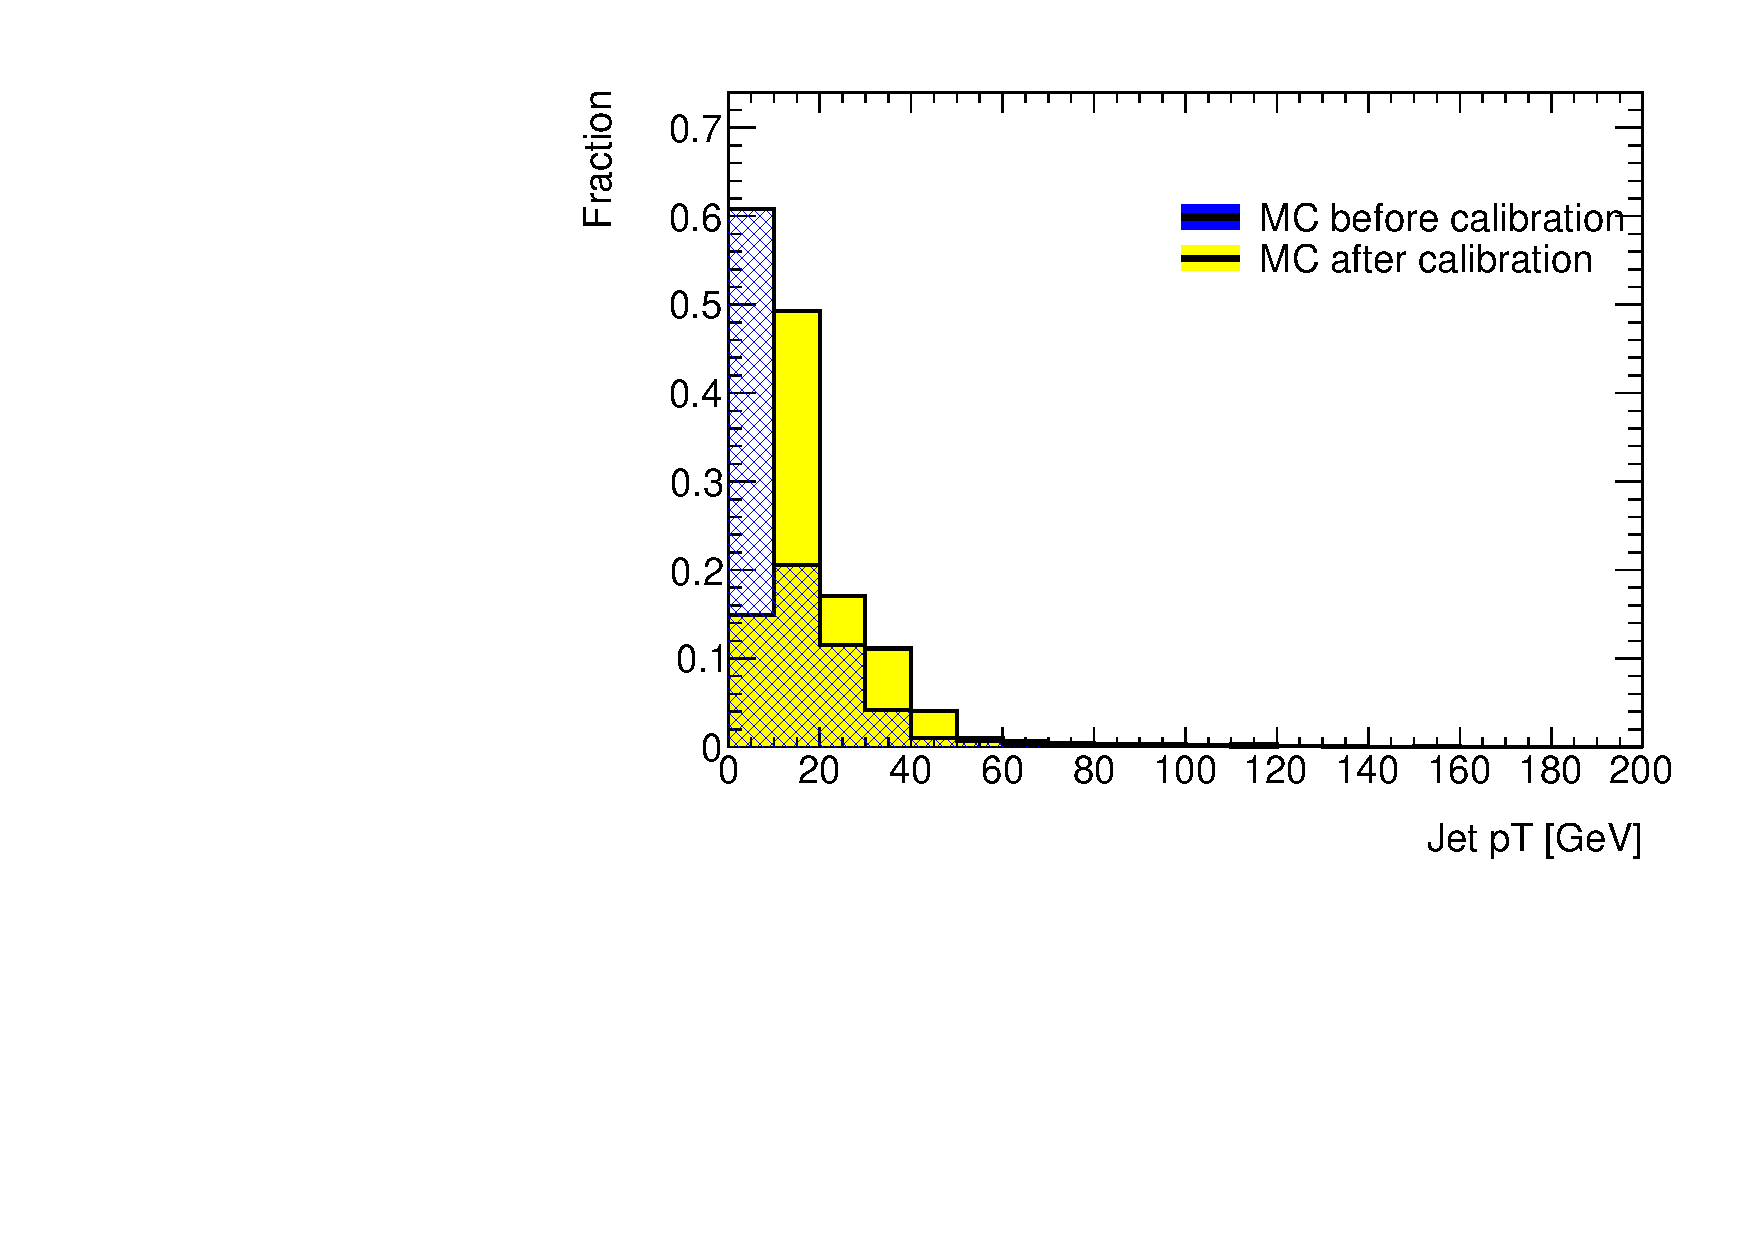
\includegraphics[width=0.53\figwidth]{testscalingpt}
\caption[Influence of the JES on the transversal momentum]{The influence of the calibration in momentum is shown}
\label{fig:testscalingpt}
\end{subfigure}
\quad
\begin{subfigure}[b]{0.5\figwidth}
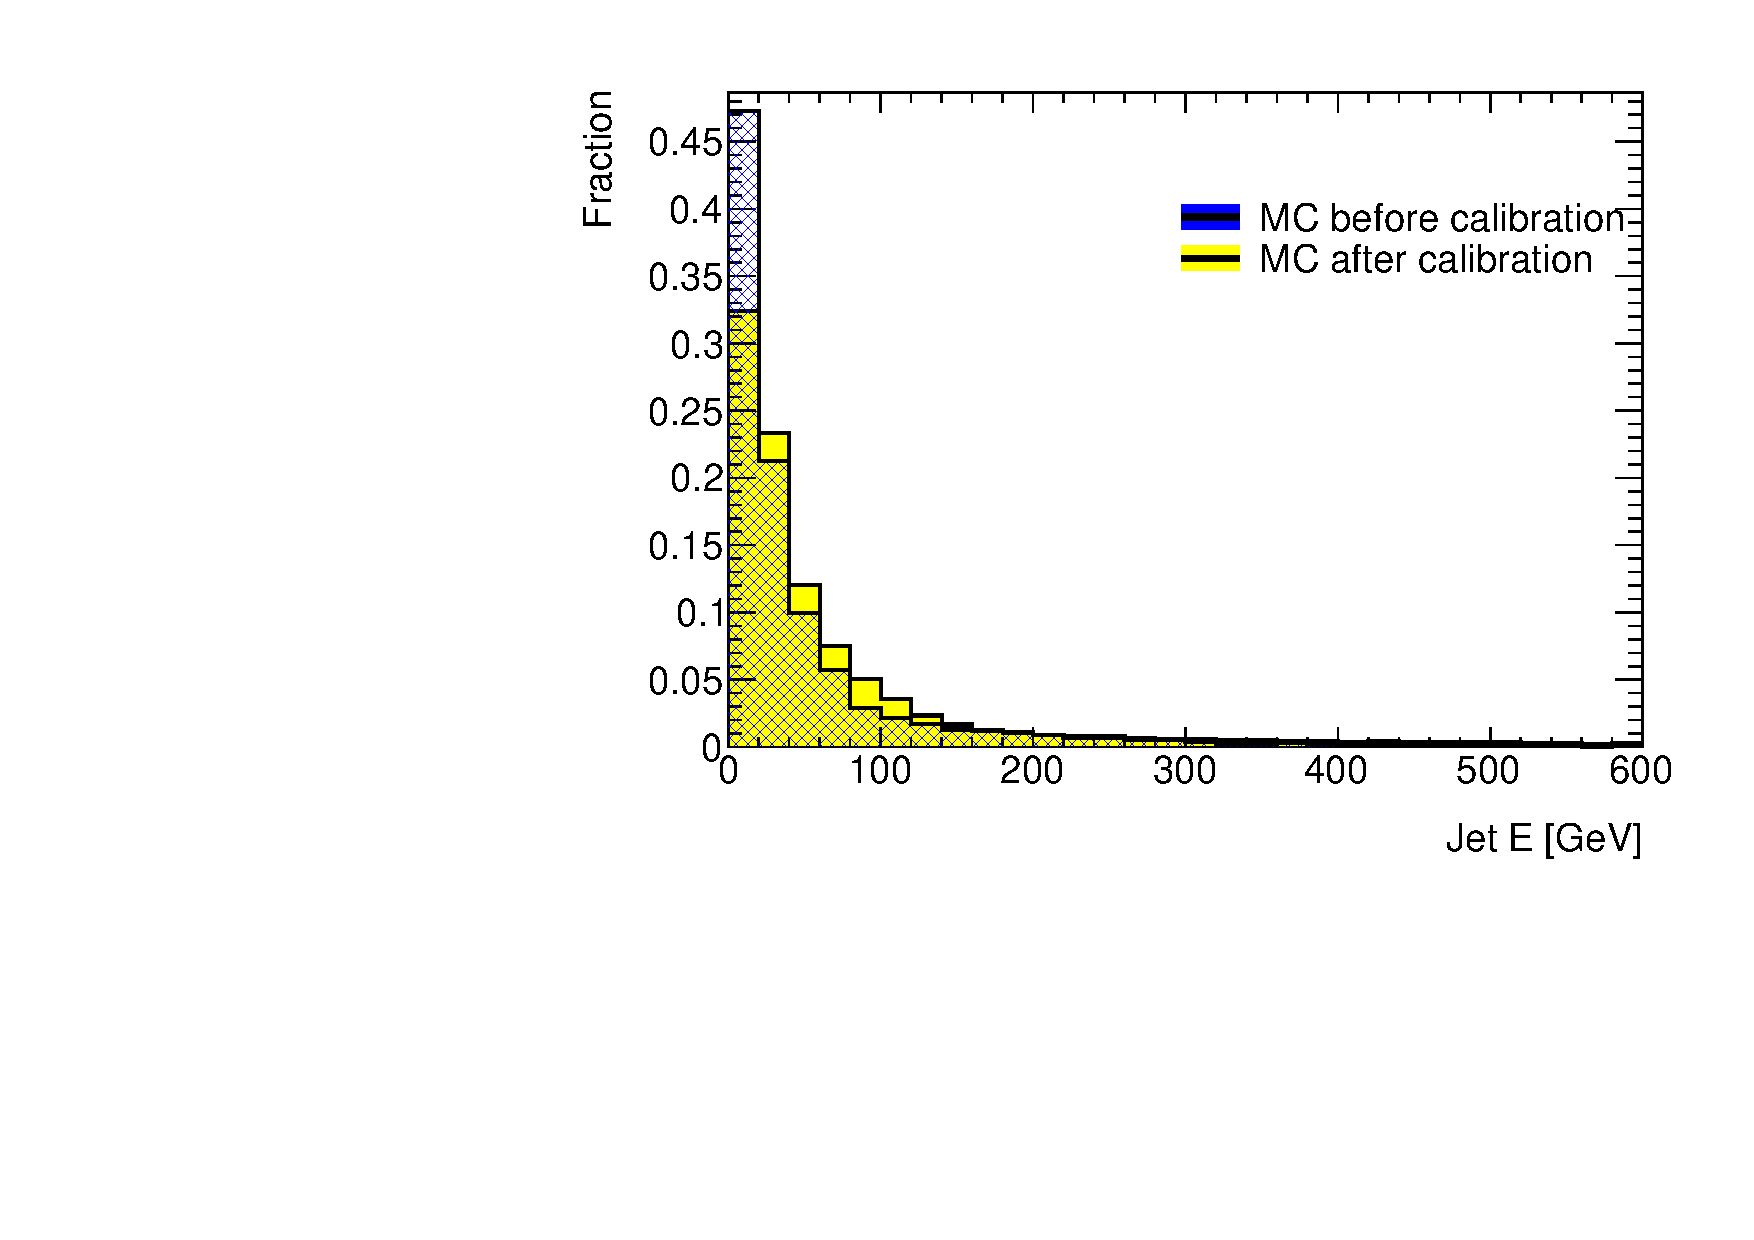
\includegraphics[width=0.53\figwidth]{testscalinge}
\caption[Influence of the JES on the energy]{The influence of the calibration in energy is shown}
\label{fig:testscalinge}
\end{subfigure}
\end{figure}


\begin{figure}
\centering
\begin{subfigure}[b]{0.5\figwidth}
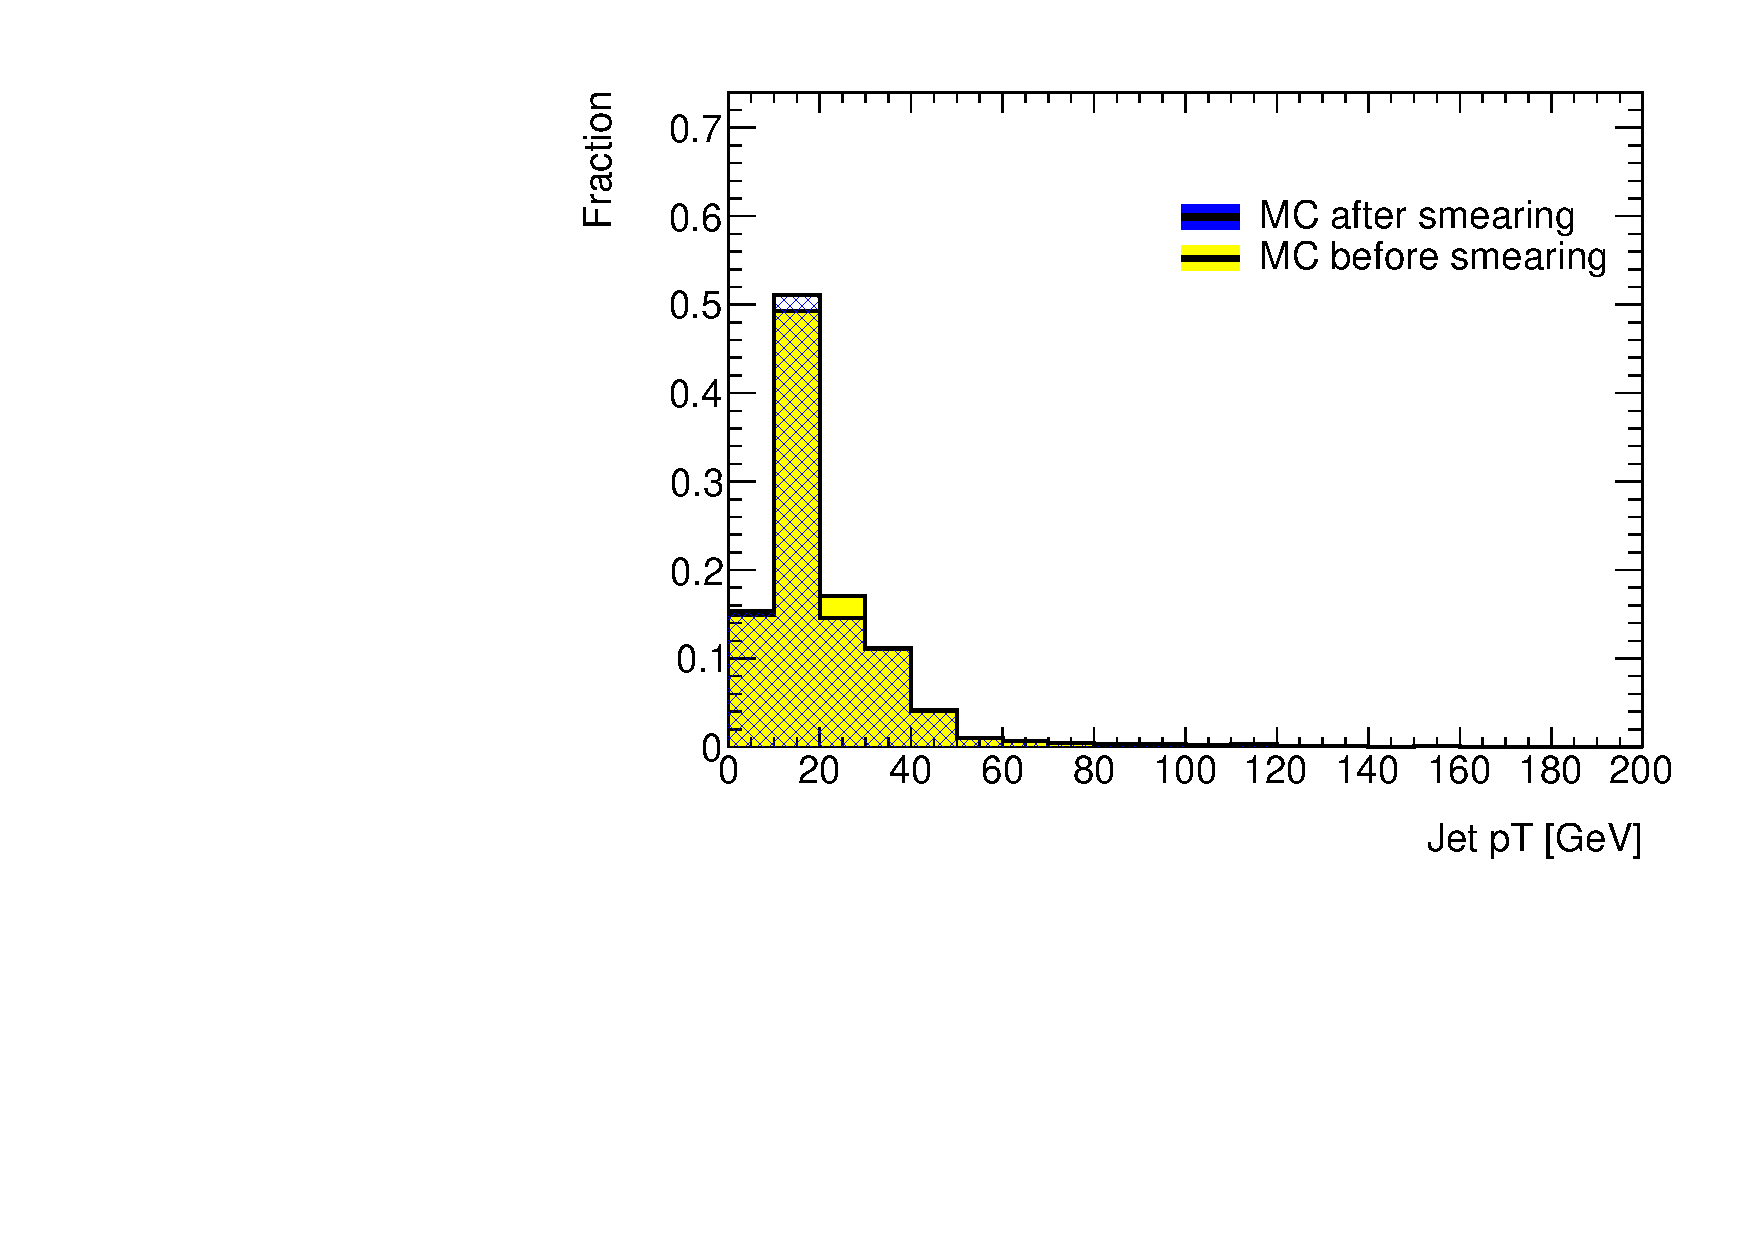
\includegraphics[width=0.53\figwidth]{testsmearingpt}
\caption[Influence of the Smearing on the transversal momentum]{The influence of the Smearing in momentum is shown}
\label{fig:testsmearingpt}
\end{subfigure}
\quad
\begin{subfigure}[b]{0.5\figwidth}
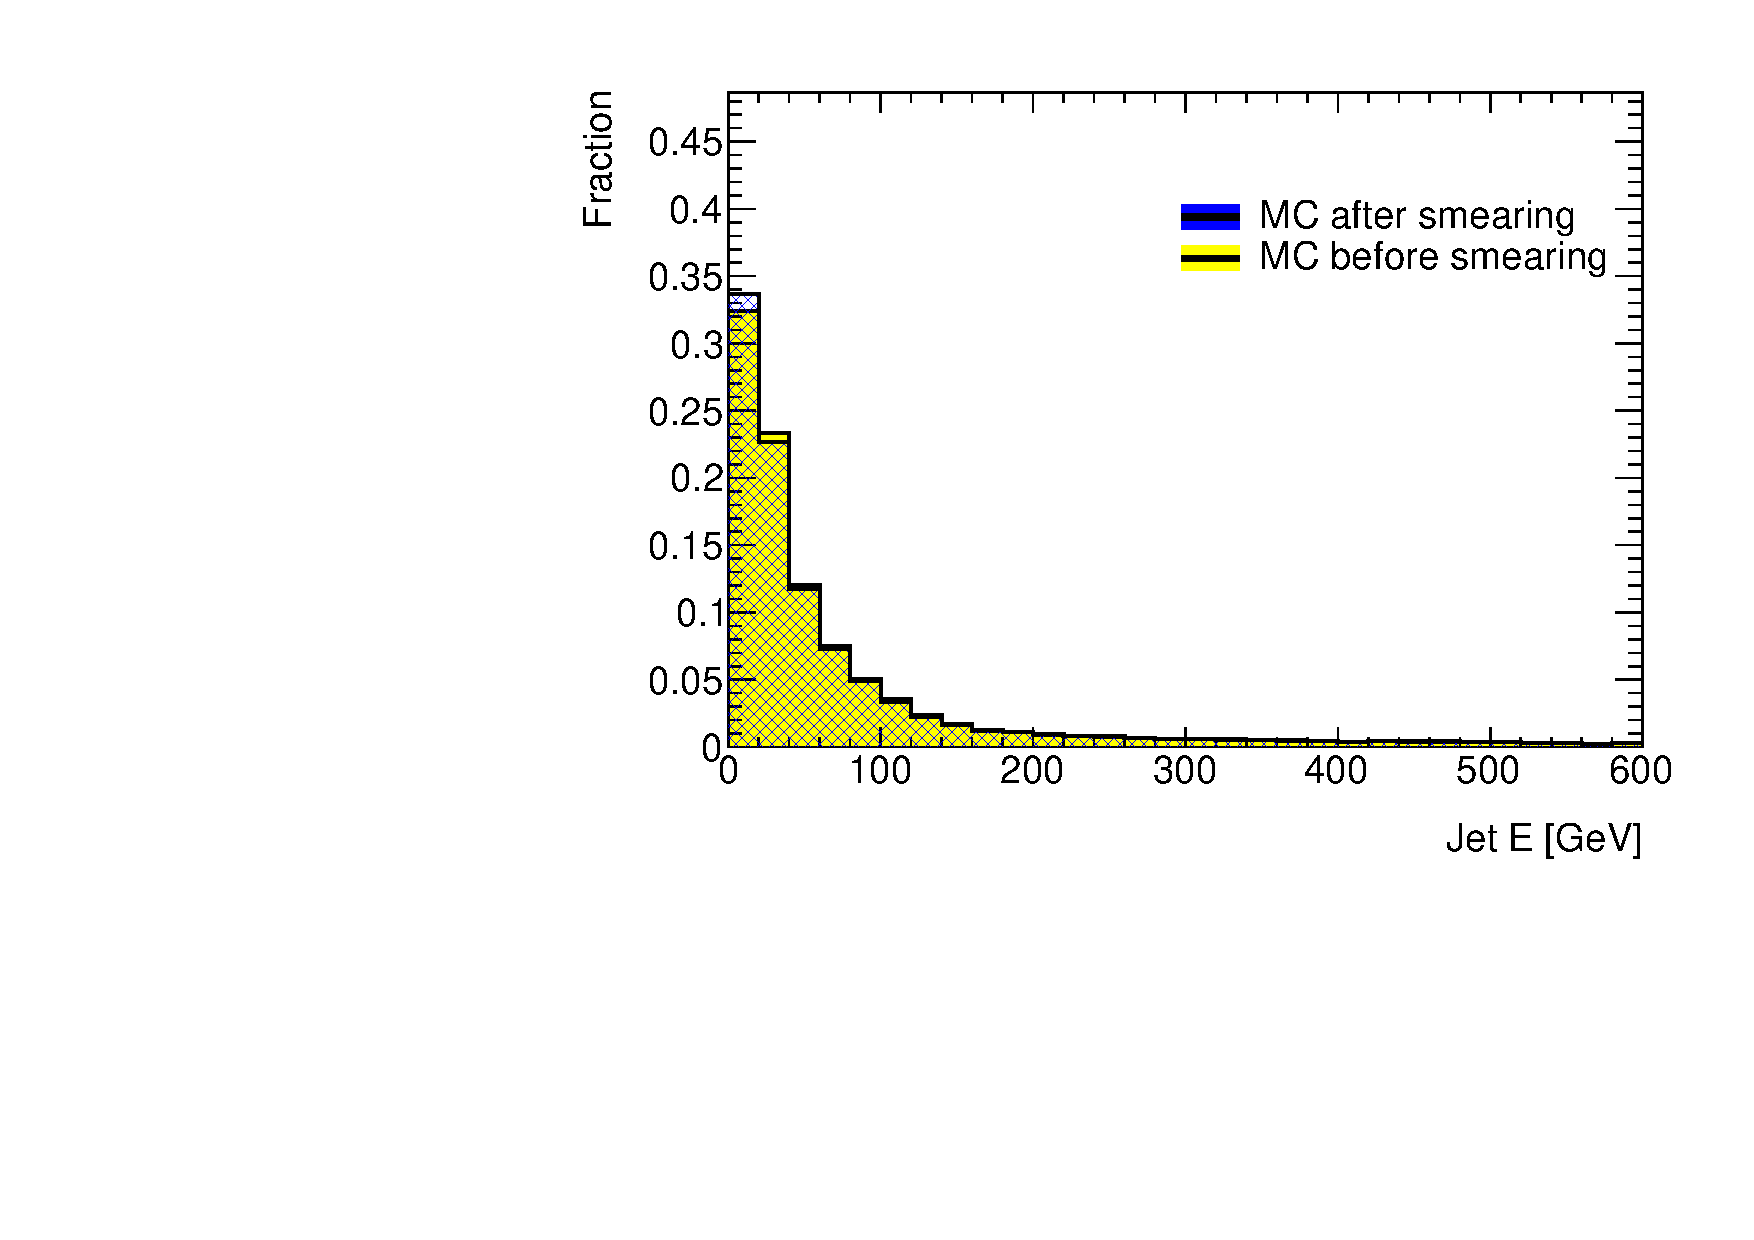
\includegraphics[width=0.53\figwidth]{testsmearinge}
\caption[Influence of the Smearing on the energy]{The influence of the Smearing in energy is shown}
\label{fig:testsmearinge}
\end{subfigure}
\end{figure}


\subsection{The jet vertex tagger}

Due to the high luminosity at the LHC in time and in space pileup is a big problem in ATLAS analysis. Therefor the rejection of pileup is an important part of analysis. One possible way to minimize pileup is to calculate the jet-vertex fraction of each jet which is the fraction of momentum in the jet originating from the primary vertex. If one sets a minimum on this fraction pileup can be suppressed because jets that do not pass the criteria on their JVF are highly likely to be originating from pileup vertices. The Jet Vertex Tagger relates each jet to a vertex.


\subsection{Muon Calibration and Selection}

Analog to jets the muons in an event also have to go through several cuts and have to be calibrated properly. This section introduces all the important tools for muon calibration and gives a brief summary of the effects of the cuts and calibrations.
The first and foremost task of the mun tools is to determine whether a muon originated from the original vertex or has its origin in background noise( cosmic muons) or in some kind of secondary interaction. Muons are reconstructed using both the muon spectrometers and the inner detector. The information from both detector systems is combined to a single track. Then the muons are requested to have $p_T > \SI{25}{\GeV}$ and a pseudorapidity of $|\eta| < \num{2.5}$. To reject the cosmic muon background further the muons are not allowed to have a longitudinal impact paramter to the primary vertex that is higher than \SI{3}{\mm}. 

The last requirement is added due to muons originating from heavy flavour quark decays.
To remove these last unwanted muons an isolation criteria is implemented, namely the isolation tool. The tool makes sure that the sum of transversal momentum of the tracks around the muon candidate divided by the muons momentum is smaller than \num{0.05}. 

\begin{equation}
\frac{\sum_{\Delta R}pT_{track}}{pT_{\mu}} < 0.05
\end{equation}

This way in $Z \rightarrow \mu^+ \mu^-$ events an efficiency of \num{97} \% in muon detection was achieved.

The second part of the muon tools makes sure that the muon properties are correctly calibrated and smeared to make Monte Carlo and data match properly and to eliminate known weaknesses in the detector structure. Figure \ref{fig:testmuonpt} shows the muons transversal momentum before and after calibration in Monte Carlo. The changes are very minor.

\begin{figure}[h]
\centering
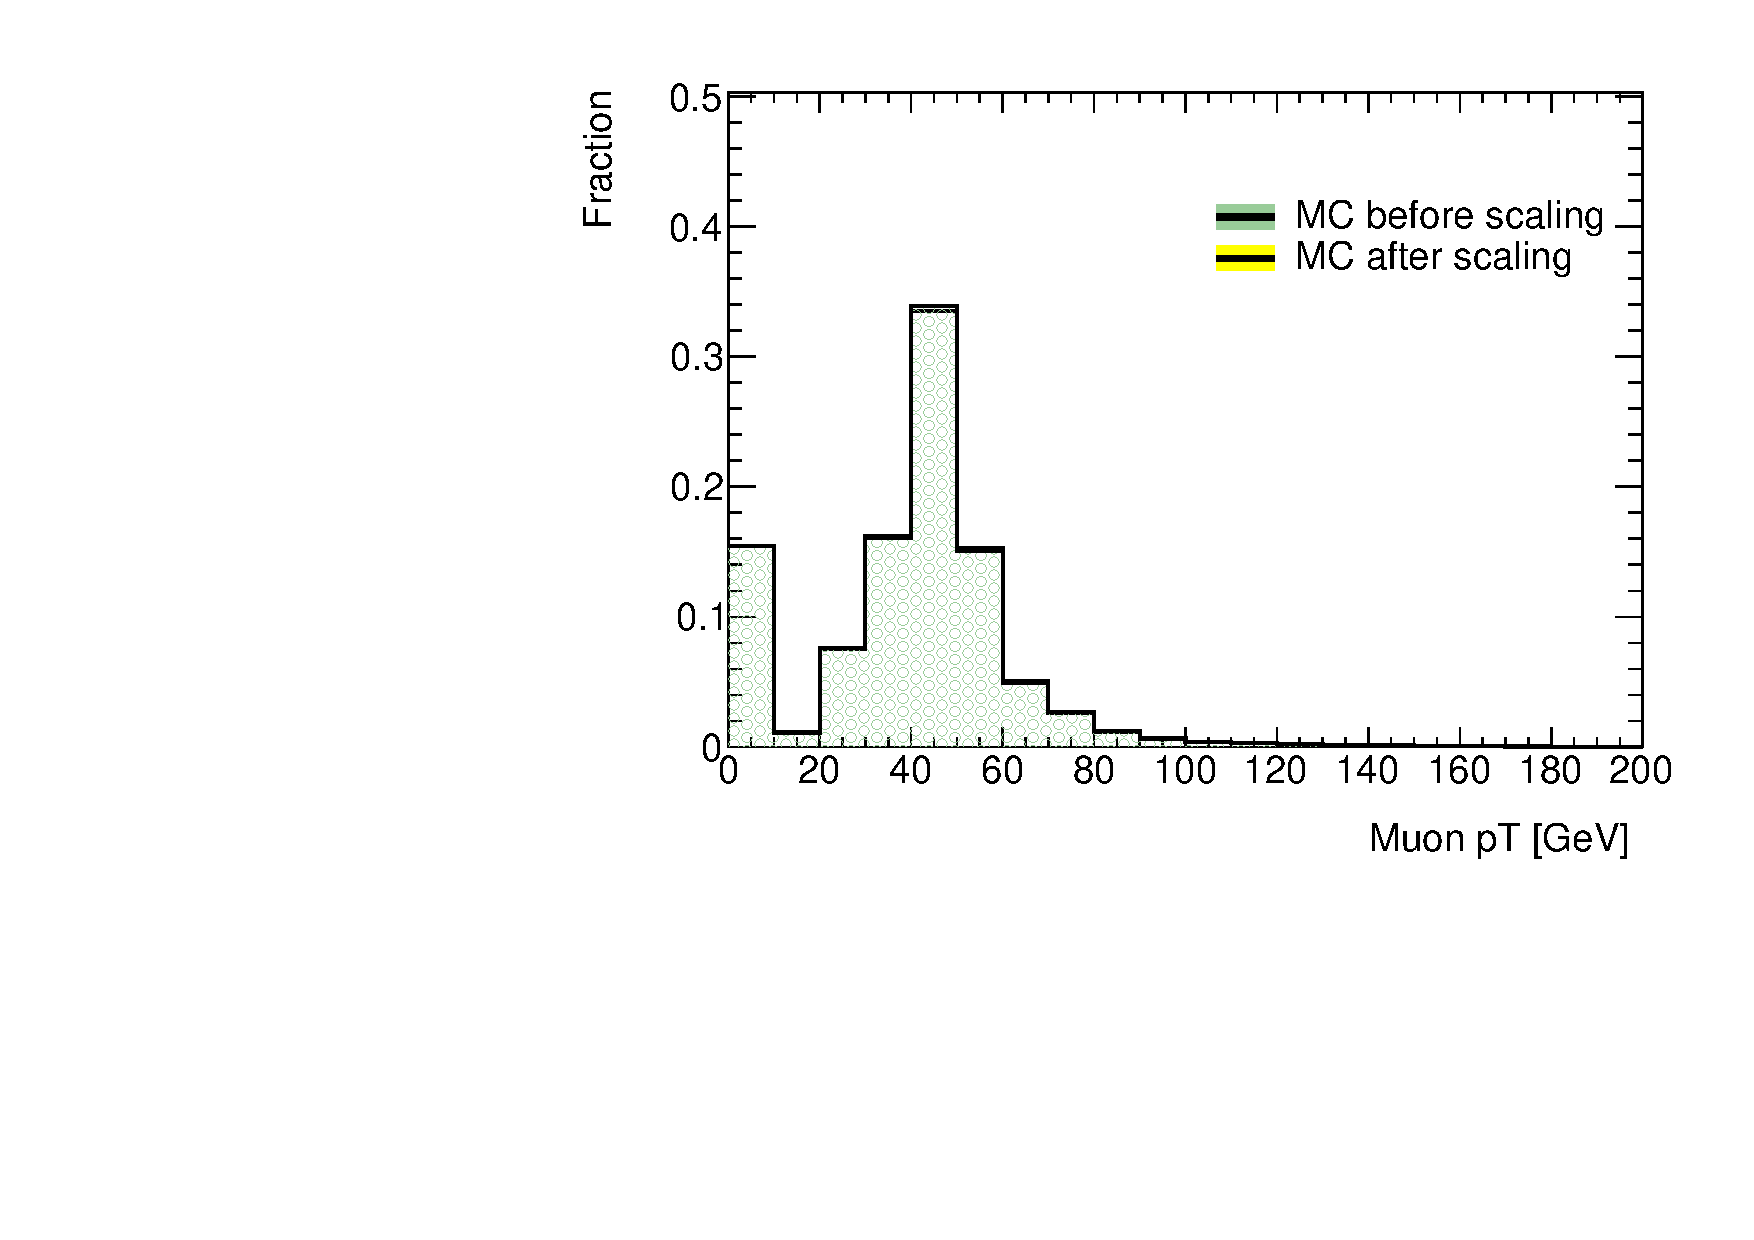
\includegraphics[scale=0.7]{testmuonpt}
\caption{Calibration and smearing of the muon momentum. The changes are very minimal.}
\label{fig:testmuonpt}
\end{figure}

\subsection{Electron Calibration and Selection}

The electron tools are the more or the less parallel to the muon tools. There is a first group of tools and criteria to determine which electrons actually originate from the primary vertex and distinguishes those electrons from background and pileup. The second group of tools calibrates the wanted electrons properties.

Electrons are detected by leaing a track in the inner detctor and depositing lose to all of their energy in the electromagnetic calorimeter. The reconstruction algorithm expects a calorimeter cluster with a deposited energy $E_T$ exceeding \SI{2.5}{\GeV}. This cluster has then to have a matching track from the primary hard scatter vertex. The $\eta$ requirements are $|\eta|_{cluster} < 2.47$ with an exclusion of $\num{1.37} < |\eta| < \num{1.52}$ (calorimter barrel-endcap transition region).

Electrons are same as muons required to be isolated. The Isolation is based on a $\Delta R < \num{0.2}$ cone in the deposited energy and a $\Delta R < \num{0.3}$ cone around the track.

The elctron calibration and smearing is exemplary diplayed in figure \ref{fig:testelectronpt}. The impact of the scaling is significantly higher than for muons.

\begin{figure}
\centering
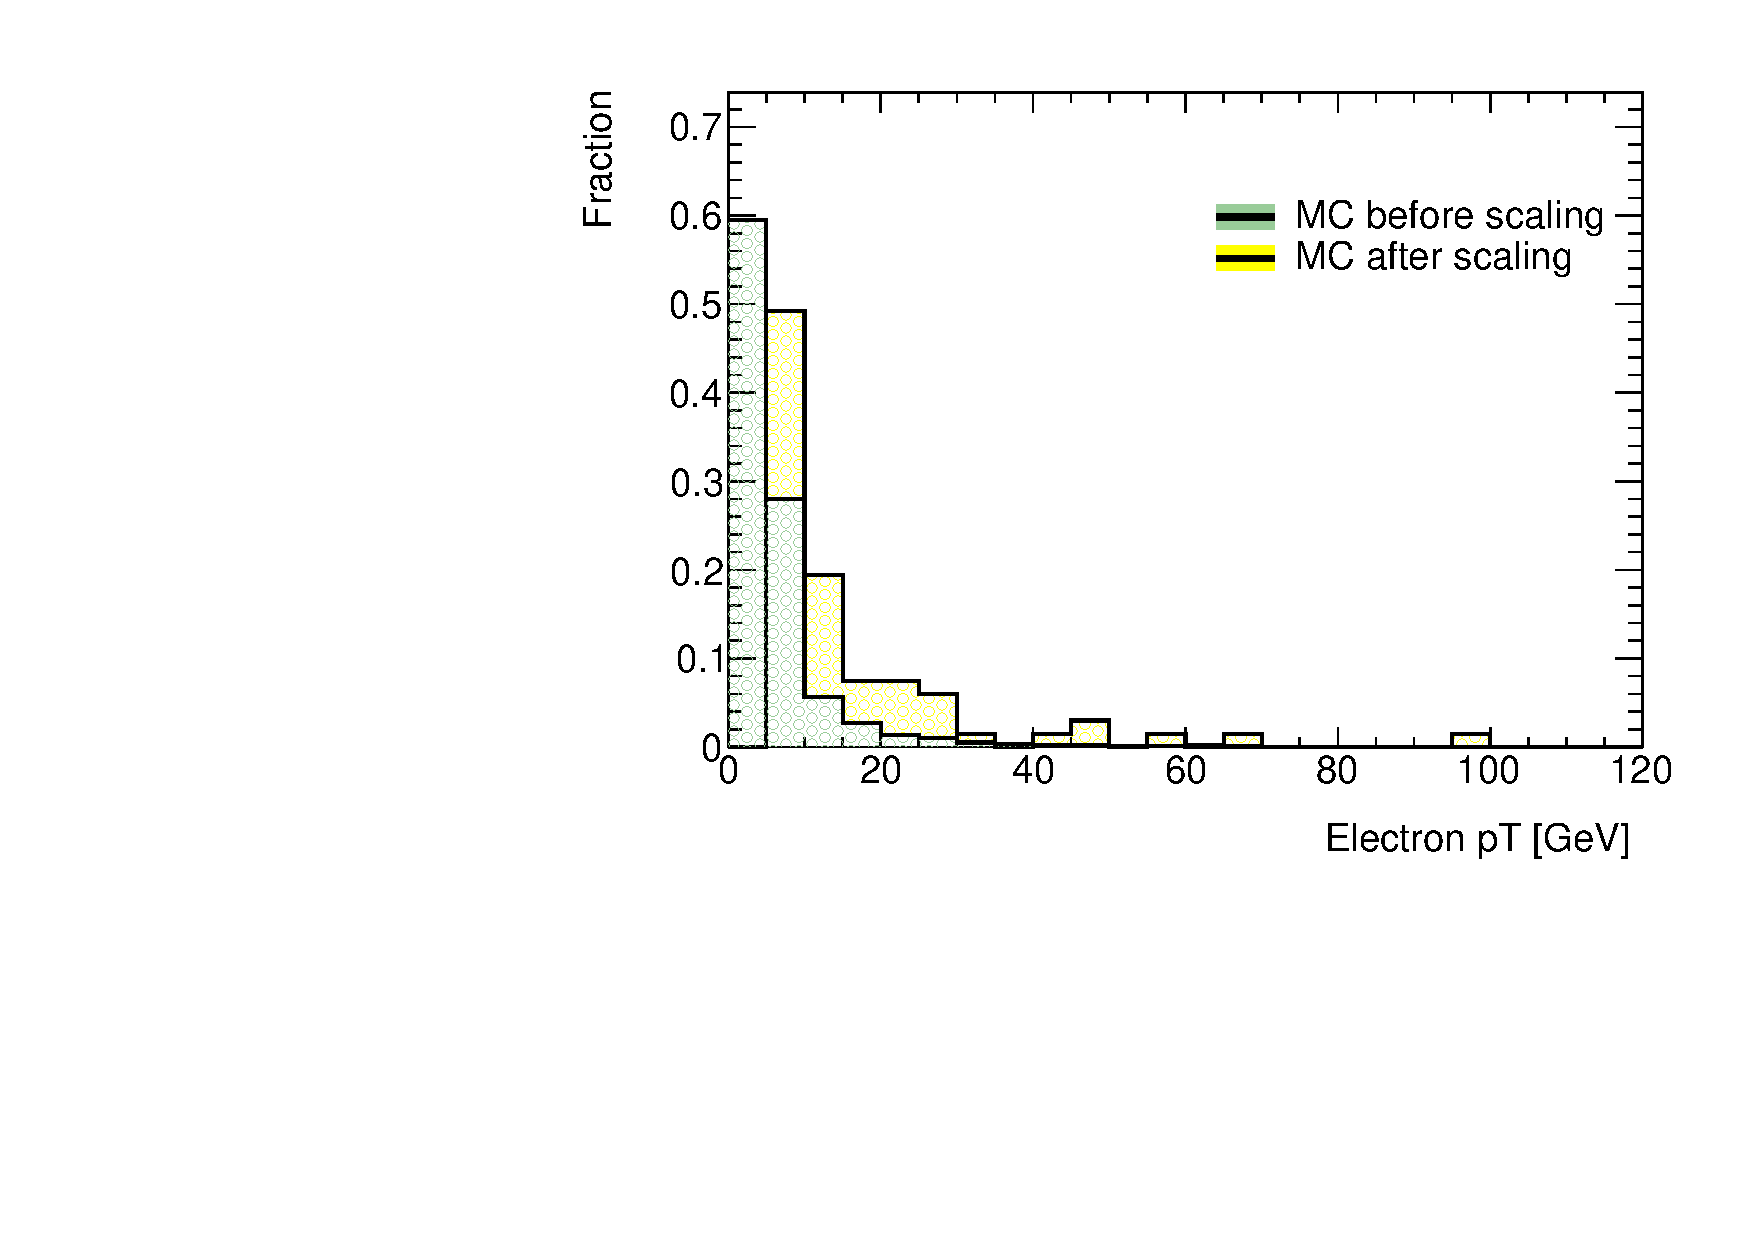
\includegraphics[scale=0.7]{testelectronpt}
\caption{Calibration and smearing of the electron momentum.}
\label{fig:testelectronpt}
\end{figure}